% This is the main report file

\documentclass{acm_proc_article-sp}
\usepackage[utf8]{inputenc}
\usepackage{listings}
\begin{document}

\title{Android based audience response system}
\subtitle{[Technical documentation]
%\titlenote{}
}


\numberofauthors{2}
\author{
\alignauthor 
Kim Rostgaard Christensen\\
Technical University of Denmark\\
       \email{s084283@student.dtu.dk}
\alignauthor 
Jeppe Mariager\\
Technical University of Denmark\\
       \email{s093253@student.dtu.dk}
}

\maketitle

\begin{abstract}
%Abstract; A brief summary of all of the report including the conclusion section
%but excluding the acknowledgements, references and any appendixes.
\end{abstract}
\section{Introduction}

%TODO
%elaboration of concept
%description of each figure
%provide a condidate list for template engines (eg. Stringtemplate or Freemarker)
%provide a condidate list for frameworks

\label{sec:introduction}




\section{Use cases}
%TODO multipicities - ex. class diagram
For our usage, two actors has been identified; a student and an instructor.
\begin{figure}[h]
\centering
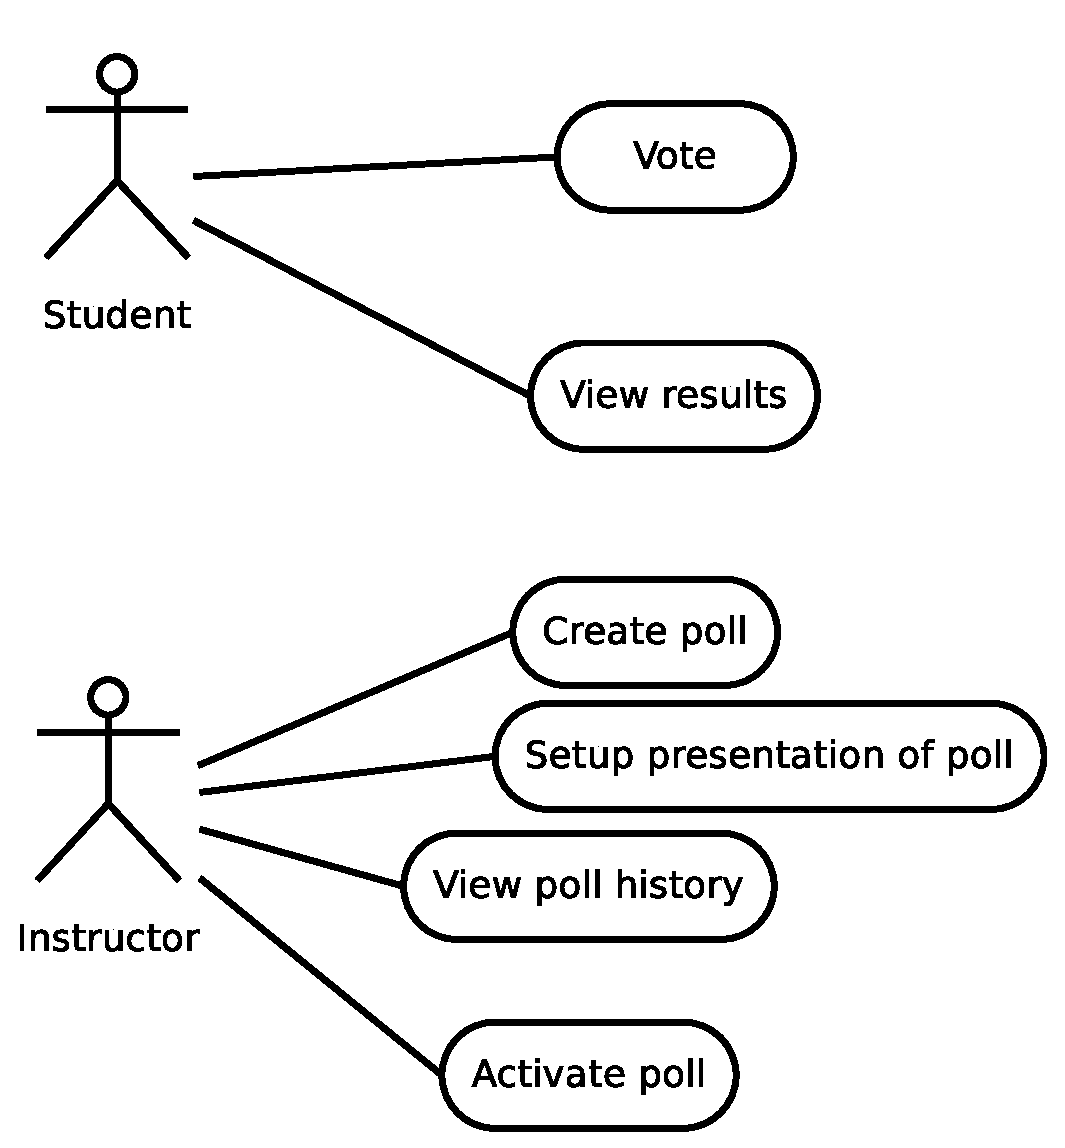
\epsfig{file=fig/use_cases.eps, height=2.0in}
\caption{Use cases}
\label{fig:use_cases}
\end{figure}
The student has access to the intended usage of the system and is considered the normal end-user. The Instructor has the administrator role in the sense that he/she is responsible for the back-office operations. For further reference, see figure \ref{fig:use_cases};

\section{Requirements}
For the system, the following requirements has been identified to support the basic usage of the system
\begin{itemize}
  \item Simple to use
  \item No user login
  \item Multiple choice polls
  \item Persistent storage of polls and results
  \item No live view
  \item Basic semantics
\end{itemize}
An elaboration of each requirement follows
\subsubsection*{Simple to use}
The system must have as little interaction with users as possible. Make as many decisions on predefined values as possible and avoid asking the user.

The system has no notion of persistent users, but instead uses a shared secret scheme in the form of a generated url. This functionality is roughly corresponding the one used at doodle.com.

\subsubsection*{Multiple choice polls}
The system is a basic multiple-choice poll. One question, several answers. Once a poll has been answered by a user, it cannot be replied to again in the same session.
%TODO Check op on this and what the conclusion on the multiple users discussion was.

\subsubsection*{Persistent storage}
The polls and the results must be stored until explicitly removed by the instructor.

\subsubsection*{No live view}
There is no live view option for showing the results before the poll closes. This is due to the fact early poll estimates can have effect on the result.

\subsubsection*{Basic semantics}
The application should a have a notion of right and wrong answers - if applicable.

\subsection{Possible improvements}
This section describes the ideas for improving the general usefulness and quality of the application.
\begin{itemize}
  \item Statistics
  \item Security and authentication
  \item Remote access 
  \item Shared voting devices 
  \item Real questions
  \item Optional user login
\end{itemize}

\subsubsection*{Statistics}
Basically any additional information that goes beyond basic usage. Comparison of results from different polls or poll sessions. This one requires the login functionality to be implemented.

\subsubsection*{Security and authentication}
More security can be added without adding extra complexity.
\subsubsection*{Remote access}
Think webcasts - no physical presense should be required
\subsubsection*{Shared devices}
More than one user has access to polls on single device
\subsubsection*{Real questions}
???
\subsubsection*{Optional user login}


%TODO
Tools used:
% - github, for revisioning og wiki
 - eclipse

\section{Infrastructure}

\begin{figure}[h]
\centering
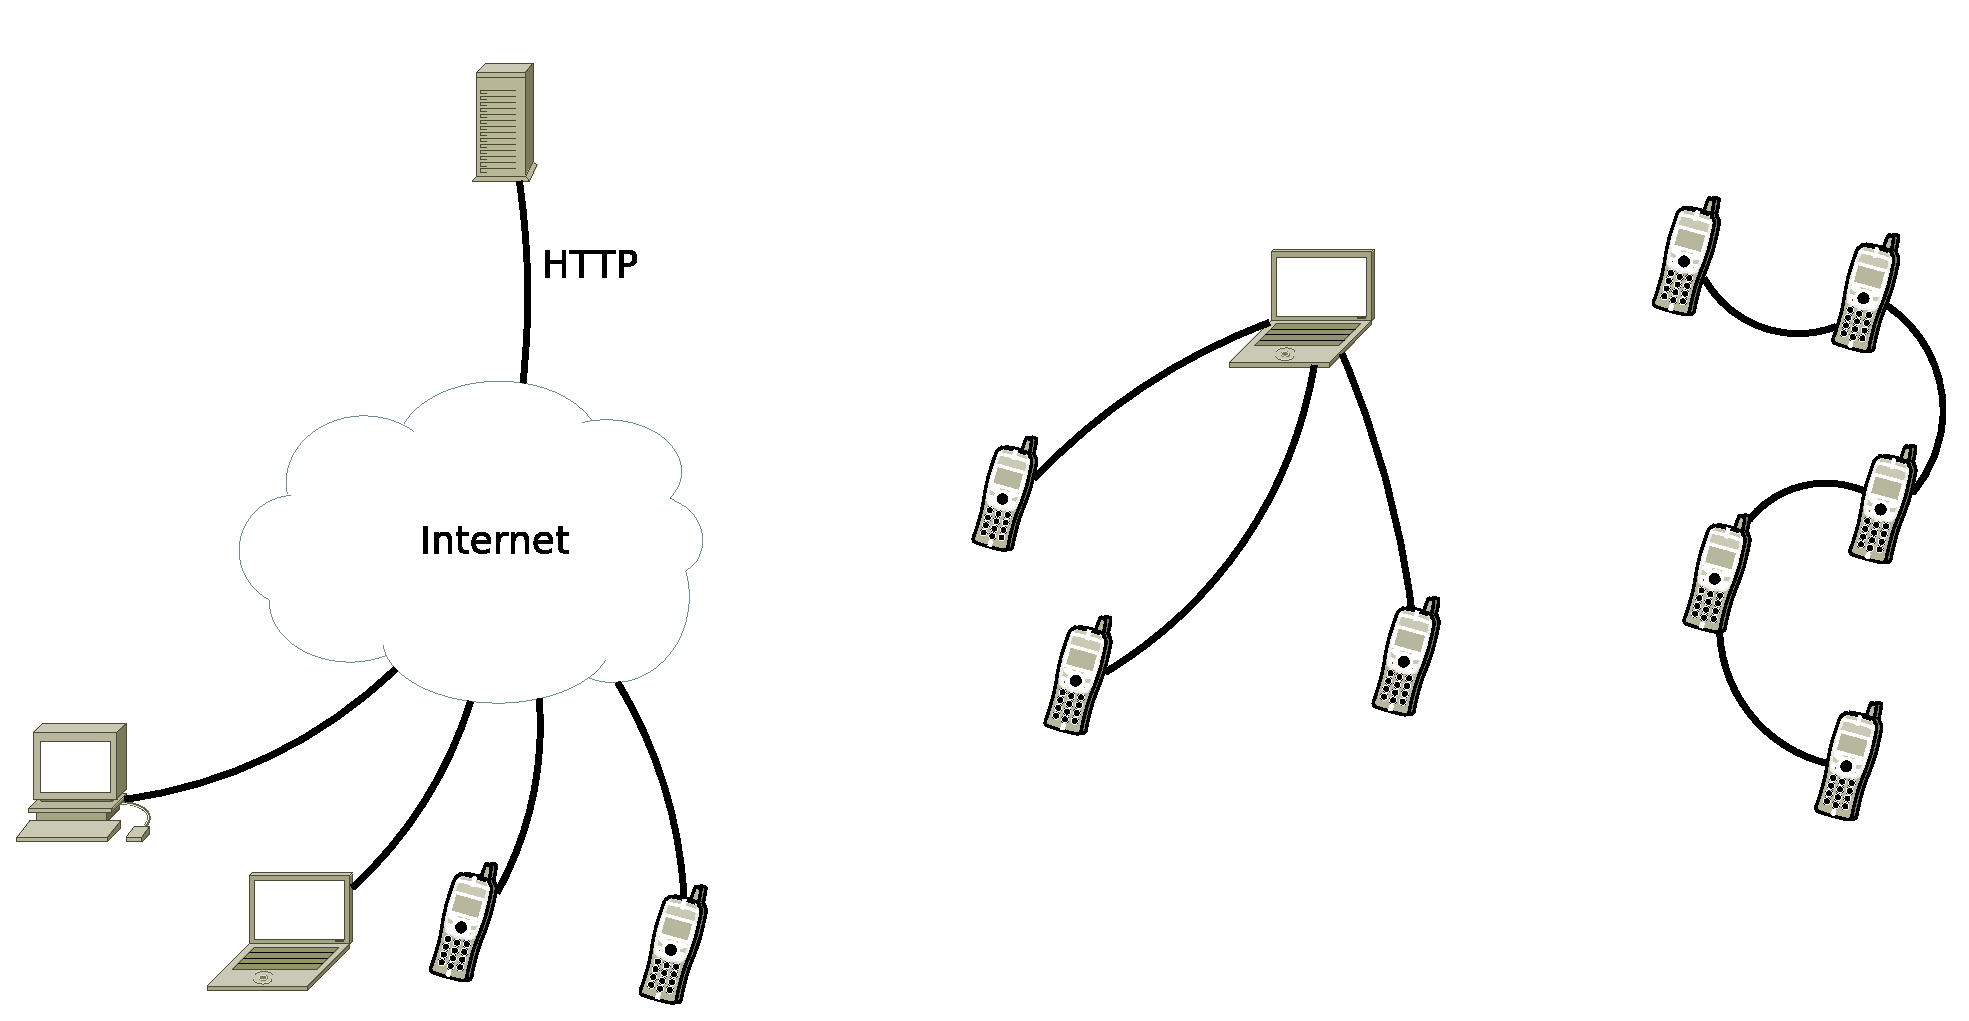
\epsfig{file=fig/architeture_choices.eps, height=1.4in}
\caption{Architeture Choices}
\label{fig:architeture_choices}
\end{figure}

For the network architecture we have chosen a classic client server setup. See diagram for options.

The mesh network was ruled out due to complications with the android ad-hoc networking not being available for non-power users.

The Ad-hoc network was rejected due to the fact that we cannot guarantee the availablilty of the service on various networks and laptops. This is caused by infrastructure security issues - e.g. local firewalls blocking zeroconf/broadcasting.

For using a laptop as access point, it is required that the application has access to the drivers of the laptop in order to change the wireless network card into managed mode. 
On a further note, we are unsure that a laptop is able to handle the number of clients required.




\section{Overall design}
\begin{figure}[h]
\centering
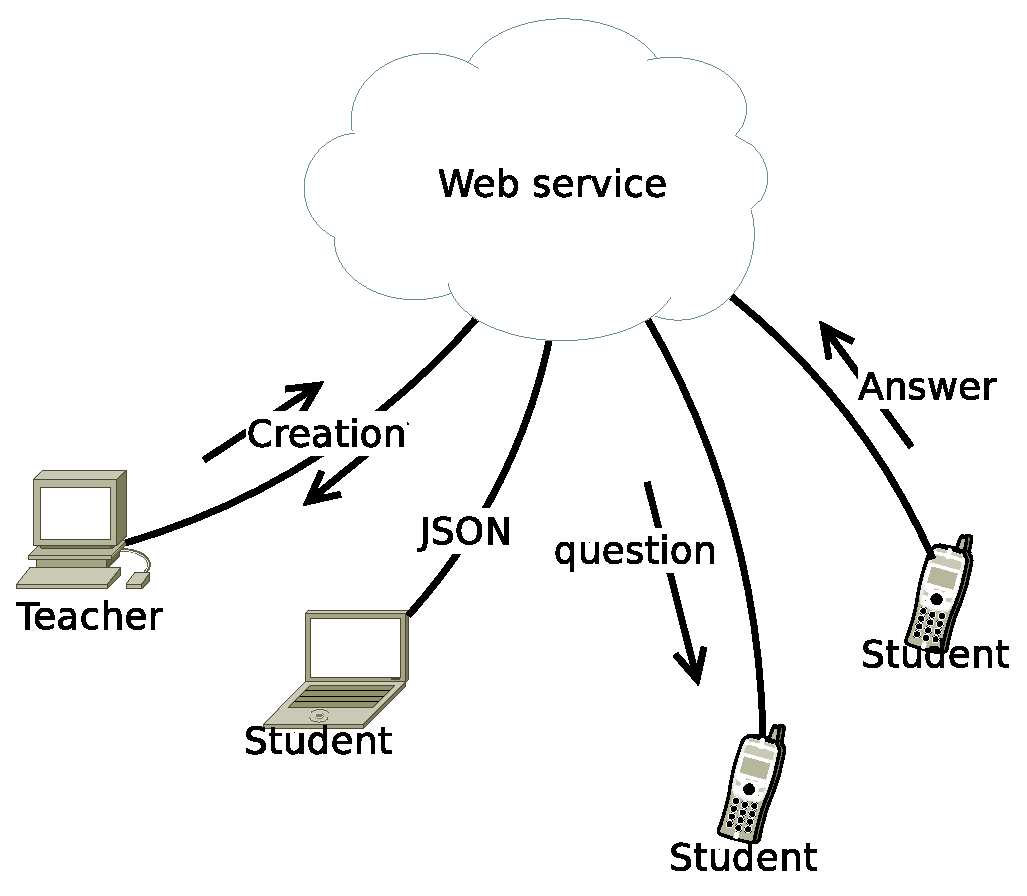
\epsfig{file=fig/web_service.eps, height=1.4in}
\caption{Web service}
\label{fig:web_service}
\end{figure}
Basically we want to do two interfaces

\begin{itemize}
  \item A client coded in AJAX that can be accesses via HTTP
  \item A client interface coded in Java for native android phones (an app)
\end{itemize}

\subsection{Protocol}

\subsection{API}


\section{Technical Requirements}
\begin{itemize}
  \item Web server with java
  \item Web server with email sending capabilities
\end{itemize}
Suggested technologies
\begin{itemize}
  \item Template engine (provide a condidate list)
  \item Some framework
  \item JSON/HTTP
  \item AJAX
\end{itemize}
 
 
\section{Discussion}
 
Security concerns/login considerations:

Student authentication is based around a unique poll ID. This ID gets generated at poll creation time. Polls can optionally be protected by a password.

The users having an android phone can access the poll (collection of questions) with the unique number supplied by the teacher. Laptop users can access the poll by putting in the same number on the webpage.

For the teacher to be able to modify the polls later in the process, an admin link is provided via email when the poll is created. This requires the teacher to supply a valid email address.

The are fuzzy thoughts about whether a device is able to vote twice, and how this is handled. A challenge respose captcha is a suggestion.


\appendix

\section{Thoughs}
Test different screen sizes

% The following two commands are all you need in the
% initial runs of your .tex file to
% produce the bibliography for the citations in your paper.
\bibliographystyle{plain}
%\nocite{*}
\bibliography{sigproc}  % sigproc.bib is the name of the Bibliography in this case
% You must have a proper ".bib" file
%  and remember to run:
% latex bibtex latex latex
% to resolve all references
%
% ACM needs 'a single self-contained file'!
%
%APPENDICES are optional


%Appendixes; Appendixes holds, for example, results or figures that are not
%relevant to place in the body of the report. Appendixes should generally be
%avoided and might not be read by the course staff.


\end{document}
